\IEEEcompsoctitleabstractindextext{%
\begin{abstract}
An electronic circuit simulator was developed to aid in the
teaching of elementary electrical principles.
It allows users to design and evaluate arbitrarily complex
circuits constrained only by the space available. The circuit is
analysed in real-time and the voltage and current levels are
displayed dynamically and intuitively by the models
representing the circuit components and their wiring.
\end{abstract}
}
\maketitle
\IEEEdisplaynotcompsoctitleabstractindextext
\IEEEpeerreviewmaketitle
\section{Introduction}
%Highlevel project description
%motivation
%learning and augmented reality

\IEEEPARstart{D}{ynamic Analysis} bitches

\section{Related Work}
Summarise related works
\subsection{Augmented Reality for Teaching Spatial Relations}
In this paper\cite{Maier09} the authors describe their tool Augmented Chemical Reactions, which is aimed at using AR to teach students about how the geometry of molecules effect reactions between them. Molecules are spatially registered to fiducial markers. Marker-cubes can be used to allow the user to view the molecule from any angle. When the markers of two molecules with the ability to bond to each other come into proximity to each other, possible bonds are shown as transparent tubes. The user can then bond the molecules if they wish.

\subsubsection{Critique}
This paper did not show complex examples or discuss in great depth the usage of their tool. This was partly due to the length of the submission, but also partly to a lack of conciseness in describing supporting topics such as the motivation and Augmented Reality, and partly to superficial explanations. The lack of detail was especially important as the tool's use for scientists designing molecules was emphasised. No mention was given to the underlying physics simulator, or the limitations of molecule numbers or complexity, which would be important information for an interested scientist. In addition, the usage in a classroom was not discussed.

An area for further work not mentioned in the paper could be integrating extra visualisations of the chemical reaction at the visible scale. A common problem with advanced concepts is the difficulty with bridging the gap between abstract concepts and real-world observations. This tool could allow a macroscopic view demonstrating the tangible outputs of a reaction alongside the individual molecule view. Extra data such as temperature and state-changes could be shown to give a more complete understanding of the reaction.

\subsection{Construct3D}
Construct3D is an AR educational tool described in the paper "Mathematics And Geometry Education With Collaborative Augmented Reality"\cite{Kaufmann03}. Using one of a number of suggested hardware set-ups, users create geometric entities such as curves and spheres using a 6 degrees-of-freedom 'stylus' and the Personal Interaction Panel, an AR interaction system\cite{szal97}. With their geometric entities they can then investigate concepts such as geometric sections and vectors. In the more ambitious hardware set-ups, users can walk around and through the geometry they create. The geometry exists on 3D layers, allowing different visibility modes for different users or teaching scenarios.

\subsubsection{Relevance}
Collaboration is emphasised, with the tool featuring shared scene-graphs and AR applications between hardware systems. This advanced form of collaboration with multiple communicating systems is not within the scope of our project, however the simpler collaboration which a single system can support is. While the educational content is not as closely related to our project, the design considerations regarding educational use are highly relevant.

\subsubsection{Critique}
The contexts in which Construct3D would be likely used for were well considered, including the possible participants and the available resources. This means that collaboration at different scales and usage through different mediums such as HMDs and monitors were designed for. An initial trial study showed that students found the tool very useful, and the tool was improved based on feedback. Large-scale studies on the educational benefits were carried out, and are summarised in a paper from 2007\cite{Kaufmann07}. Many improvements were made based on the results of these studies.

\subsection{Understanding Ohm's law - Enlightenment Through Augmented Reality}
In this paper\cite{peng2010understanding}, authors Peng and M\"{u}ller-Wittig discuss a system that allows a user to interactively build circuits via the placement of fiducial markers. The markers represent resistors, which are displayed with their colour coded stripes showing.

The surface onto which the markers are placed has a fixed set of component slots. The user needs to place enough markers into these slots to make a complete circuit. At this point the user sees a wire rendered around the circuit, the software calculates the total resistance of the circuit and consequently the current which must be flowing through a bulb which is connected in series with a virtual DC power supply.

The bulb is a real light source, driven by a DC supply and interfaced to the computer via an Arduino development board. It is the only source of feedback provided to the user barring the textual information presented to the user in a dialogue box.

Peng and M\"{u}ller-Wittig's paper also provides some insight into the relevance and efficacy of augmented reality applications as teaching tools and the cost benefits of doing so.

\subsubsection{Relevance}
This project's goals are very similar to our own, if somewhat limited in their scope. As such this project makes an excellent starting point for us and its method and results are worthy of note.

Similarities:
\begin{itemize}
\item A single web camera is all that is required for input into the system, although there is no reason either system may not be improved with a more complicated set up, such as a head mounted display.
\item Fiducial markers are used to represent the location of the components they represent. Those components are displayed above the marker.
\item OpenSceneGraph is used to build the virtual part of the scene.
\end{itemize}

We do, however, plan to expand on the number of different components available, their use of static models for components and their lack of feedback through augmented reality.

\subsubsection{Criticism}
The system appeared to be very simple to use and may be an effective teaching tool. It was limited, however, in the following areas.
\begin{itemize}
\item The user receives feedback from the circuit only through the bulb. The system could be expanded to show the effects of voltage division.
\item Their use of fixed slots limits the user to a few simple circuits. This feature does make it easier to calculate voltages and allows the user to more easily distinguish between components which are in the circuit and which are out.
\item The results of the simulation's calculations are displayed in a dialogue box on screen, they could have attempted to display information over the component it pertains to.
\end{itemize}

\subsection{Motion in Augmented Reality Games: An Engine for Creating Plausible Physical Interactions in Augmented Reality Games}

Namee et al\cite{namee2010motion} have developed a game engine for interactive augmented reality gaming. The engine is modular in design, it contains a World Model, an AR Registration Engine, a Physics Engine and a Renderer.

They implemented the Registration module with the ARToolkit API, the Physics module with the Open Dynamics Engine and Havok, and the renderer with OpenGL. As they point out though, MARG is technology agnostic and the implementations is not that important; the paper's focus is on software abstraction, design and the two proof of concept applications.

Objects in the Motion in Augmented Reality Games (MARG) engine can be virtual, physical or a combination and they always have an associated physics model.

Two concept games were developed by the team to demonstrate the engine's ability to handle interactions between physical and virtual objects. To show how well the user's expectations of the outcomes of these interactions are met, the team timed participants completing simple challenges using both the AR games and matching games made of entirely physical components. Although the completion times were greater and had more spread for the AR versions the times were still comparable
showing that MARG can integrate virtual objects with physical ones believably.

\subsection{Relevance}
The top level design of MARG is very similar to the design of our software, if the mechanical physics engine is replaced with an electrical physics engine/simulator then the software meets our needs completely. That is to say in both our project and theirs the user controls physical and virtual objects in 3D space and those objects are modelled by a physics engine.

\subsection{Critique}
MARG's well thought out design allows quite a bit of flexibility in terms of what may be implemented. Their two example games demonstrate the full power of MARG.

The results of their user tests appear to show MARG being slightly more difficult to use than an equivalent physical system yet they do not explore the cause of this.


\section{Project Goals}

This goals of this project were to use AR to provide a novel electricity education tool. Users build virtual electronic circuits and the states of the electrical components are visually represented. To achieve this, the following general goals were set:

\begin{itemize}
\item Represent various electrical components with some real-world object, each corresponding to a single marker.
\item Allow users to create and destroy connections between components using some intuitive interaction.
\item Visualise this connection.
\item Simulate the current through and voltage drop of each component.
\item Visualise this data.
\end{itemize}

Once the approach for solving these goals had been planned, a set of more specific goals for producing incrementally more challenging interactions and physical modelling were created:

\begin{itemize}
\item To test connection interactions, demonstrate a battery and lamp circuit.
\item To test logical circuitry modelling and extended interactions, demonstrate a logic circuit where the user can change input states.
\item To test the completed physics simulator and the current and voltage visualisations, demonstrate an AC circuit with the current and voltage represented as a pipe above the circuit.
\end{itemize}

\section{System Description}
The entire system was comprised of software running on a pc,
a single camera which was fixed or free at the user's discretion,
and a set of markers representing the circuit components which
could be laid out on any flat surface.

\subsection{Software}
The application was developed using the the OpenSceneGraph library
(which uses OpenGL) for 3D graphics, AR Toolkit for marker
tracking, and the libconfig library to simplify settings and
allowing the user to change soft parameters. Gnucap, a commandline,
open-source circuit simulator was modified into a library an
integrated into the project as well.

The software structure, starting at the top, can be simplified into
the following hierarchichal model.

\begin{verbatim}
Circuit
   -- Scene (resistor)
      -- Fiducial marker identifier
      -- OSG 3D model
      -- Gnucap component
      -- Wire models
         -- 3D model
         -- 2 scene references
   -- Scene (supply)
      -- Same as above...
   -- etc.
\end{verbatim}

Hence each scene is responsible for maintaining the electrical, graphical
and spatial states of a single component. Each scene also owns a set of
wires of a variable size. During each iteration components check for
proximity between their leads and the leads of other component, adding
and removing wires as necessary. The circuit object which requests these
proximity checks enforces that each combination of scenes is only checked
once (e.g. ab == ba) to avoid duplicate wires being instantiated.

\subsubsection{OpenSceneGraph}
OpenSceneGraph provides am application programming interface to a powerful,
OpenGL backed, 3D graphics engine. As the graphics requirements of the AR
Circuits application were not very large, our interactions with this
library were limited to importing models created in the Maya 3D modelling suite,
generating simple geometric shapes programmatically (for wires and leads), and
transforming all of these models according to marker location found using AR
Toolkit.

\subsubsection{AR Toolkit}

\subsubsection{Libconfig}

\subsubsection{Gnucap}

\section{User Interaction}
Marker set (link to config files).
Single camera.

User interaction modes.

\begin{figure}
\begin{center}
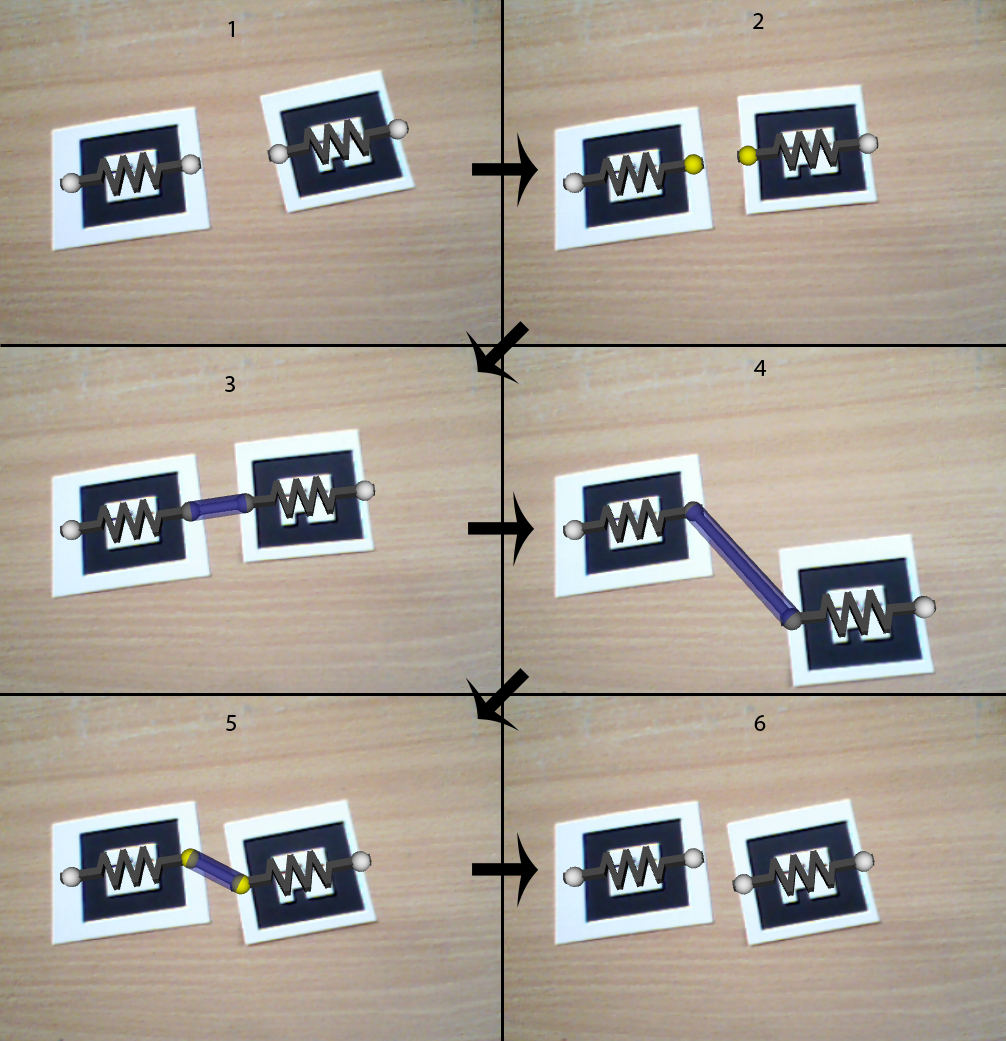
\includegraphics[width=0.50\textwidth]{connection}
\end{center}
\caption{The connection toggling process}
\end{figure}

\section{Discussion}

When the user is building the circuit and a marker is lost, the wires for that component are 
[[Dealing with losing part of the circuit, all of the circuit.]]

As with most interactive AR systems, incorrect occlusion of the real world by the digital content is an issue. When a user moves their hand to a position which should be in front of the 3D content (without blocking the marker) the content is drawn in front, as the graphics system does not have any depth information aside from the relative position of the marker. This reduces the believability of the system and can be confusing to view. Various methods of depth detection, are available which can be used to provide roughly correct occlusion. However they require extra hardware and the results are often noisy, so that the digital content appears to have frayed edges where it meets with the real-world object. For these reasons, it was decided not to use occlusion.

Each marker corresponds to a single component, and the expected use is for the marker image to be representative of the component. This limits the number of markers, and hence components, which can be viewed at once. An alternative to this paradigm is demonstrated by the Augmented Chemistry project \cite{fjeld07}, which uses AR to teach organic chemistry. One marker represents the molecule under construction and another is used to bring in new atoms to be added to the molecule. A book of markers, each representing an atom, is used to select which atom is being added. Using this interaction paradigm the number of components would not be constrained by the number of markers. However, in electronics only the connections are important, not the layout, whereas in chemistry the layout is fixed. A useful ability for understanding electronic circuits is being able to rearrange the layout of components, which the Augmented Chemistry paradigm does not easily allow.


\subsection{Limitations}


The number of markers which can be viewed at once is limited by the resolution of the camera, as the markers will not track if they appear as too few pixels in area to the camera

One challenge with all visualisations is dealing with different data ranges. Currently, no automatic scaling of voltage and current values is implemented. This means that the user must choose component values which result in values in a certain range, or the visualisation will not be easily visible.

\section{Further Work}

A common approach to real circuit analysis is to use a test probe to measure electrical information at various points around a circuit. To emulate this interaction, a tangible probing prop could be tracked which shows electrical information about a component's lead, when brought into proximity of that lead. The information could be displayed in a separate window on the computer (when the main output is not full screen) or could be integrated into the main view, with waves being displayed above the wires, or even as the wires.

The voltage-current visualisation could be improved. One possibility is integrating it with the wires that connect components. This might be more intuitive, as the relationship between current, voltage and the wire is more explicit, but it also might be confusing to view, especially with AC flows, as the heights of the components would all be changing constantly. For some viewers this might enhance the experience, while for others it might confuse it, so allowing the user to choose from both visualisations might be preferable.

Gestures could be added to improve interaction. Shaking a marker could toggle the component into and out of edit mode. `Shaking' would be defined as fast movement from side to side relative to other markers, rather than relative to the camera. This prevents camera shaking from falsely causing interaction. This would require three markers to be visible to determine the which marker was moving, unless some form of optical flow was added to detect background movement. In edit mode moving a marker vertically could cause its component to grow and shrink, and moving it horizontally could cause its primary parameter to change. An alternative could be using a special marker to alter the parameters or marker size.

To improve the scalability of the system, a circuit block element could be added. The user could build up a circuit and then assign it to a special marker as a single item. When the special marker is brought close to a component, instead of connecting to the component it would `absorb' all connected components. Since the resulting composite component might contain many connectable nodes and these nodes will be closely packed, the connecting process should use a ``connect to closest'' rule to avoid making multiple connections at once. To edit the composite component, the user would shake the marker, at which point all other components disappear and the original markers used to make the composite component would be used to make changes.


\section{Conclusion}

